\section{Durchführung}
\label{sec:Durchführung}
    Für die Versuchsdurchführung wird eine transparente Grundplatte verwendet.
    Auf dieser befinden sich zwei Laserdiodenmodule, die im Halbkreis verschiebbar sind.
    Auf der anderen Seite ist ein Reflexionsschirm montiert, zum Schutz vor das Laserlicht.
    Der Schirm ist zweiteilig, somit kann ein Teil dazugesetzt oder entfernt werden um dadurch die Höhe des Schirms zu variieren.
    Im Folgenden werden beide Teile des Schirms über den ganzen Versuch verwendet.
    Bei den beiden Lasern handelt es sich einmal um rotes Licht mit einer Wellenlänge von $\lambda = \SI{635}{\nano\metre}$ und einmal
    um grünes Licht mit einer Wellenlänge von $\lambda = \SI{532}{\nano\metre}$.
    Die Platte, sowie die Leutdioden und der Reflexionsschirm sind in \autoref{fig:platte} zu sehen.
    Über den ganzen Versuch hinweg ist Luft das erste Medium.
    
    \noindent
    In der Mitte der Platte können dann die verschiedenen Objekte befestigt werden.
    Im ersten Versuchsteil wird mithilfe der Reflexionsplatte das Reflexionsgesetz untersucht.
    Die nächsten beiden Versuchsteile beschäftigen sich mit dem Brechungsgesetz und dem Strahlenversatz, dazu wird die planparallele Platte verwendet.
    Danach wird die Brechung des Lichts durch das Kronglas-Prisma betrachtet.
    Und zum Schluss wird die Beugung am Gitter untersucht.
    Bis auf die Gitter sind die Objekte in \autoref{fig:objekte} zu sehen.

    \subsection{Reflexionsgesetz}
        Hier wird nur der grüne Laser verwendet.
        Mithilfe einer Halterung wird der Spiegel in die Mitte der Platte befestigt.
        Unter der Platte wird eine Vorlage geschoben mit der die Einfalls- und Ausfallswinkel abgelesen werden können.
        Nun wird die Diode bewegt und beide Winkel werden abgelesen.
        Diese Messung wird 7 Mal für verschiedene Einfallswinkel wiederholt.

    \subsection{Brechungsgesetz}
        Es wird weiterhin das grüne Licht und die Vorlage zur Winkelmessung verwendet.
        Die planparallele Platte wird eingesetzt.
        Das auftreffende Licht wird durch die planparallele Platte gebrochen, da diese auch eine Winkelskala aufgedruckt hat, kann hier der Brechungswinkel abgelesen werden.
        Der Einfallswinkel wird von der Vorlage abgelesen.
        Auch hier wird die Messung für 7 verschiedene Einfallswinkel durchgeführt.
        Dieselben Werte werden dann auch für die Berechnung des Strahlenversatzes verwendet.

    \subsection{Prisma}
        Hier wird zunächst der grüne Laser verwendet.
        Die Winkelvorlage wird gewechselt.
        Ein sogenannter Transmissionsschirm werden an das Ende der Vorlage aufgestellt.
        Da auf ihnen eine Winkelskala gedruckt ist, können die Brechungswinkel des Lichts nach Austritt des Prismas abgelesen werden.
        Nun sollen 5 verschiedene Einfallswinkel $\alpha_1$ im Bereich von $\SI{10}{\degree} \leq \alpha_1 \leq \SI{60}{\degree} $ und die dazugehörigen Ausfallswinkel $\alpha_2$ nach dem Prisma notiert werden.
        Die Messung wird für dieselben Einfallswinkel mit rotem Licht wiederholt.

    \subsection{Beugung am Gitter}
        Die Winkelvorlage bleibt dieselbe wie in dem Teil zuvor.
        Der Transmissionsschirm wird gewechselt.
        Da der grüne Laser zu niedrig ist um durch das Gitter zu strahlen, werden die Gitter und ihre Halterung nicht auf die Platte gesetzt sondern davor.
        Somit befindet sich das Gitter auf dem Tisch, direkt an der Kante der Platte.
        Die Messung wird für das grüne und rote Licht gleichzeitig durchgeführt.
        Dabei strahlt das Licht direkt auf das Gitter und wird gebeugt.
        Die verschiedenen Intensitätsmaxima $k$-ter Ordnung sowie die dazugehörigen Winkel werden notiert.
        Die Messung wird für drei verschiedene Gitter wiederholt, diese haben 100, 300 und 600 $\text{Linien}/\si{\milli\metre}$.


        \begin{figure}
            \centering
            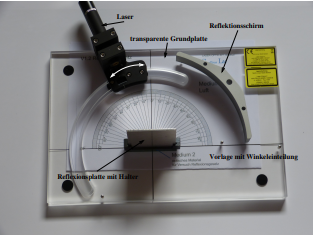
\includegraphics[width = 0.5\textwidth]{bilder/platte.PNG}
            \caption{Die transparente Platte, die Laserdioden und der Reflexionsschirm.\cite{anleitung}}
            \label{fig:platte}
        \end{figure}

        \begin{figure}
            \centering
            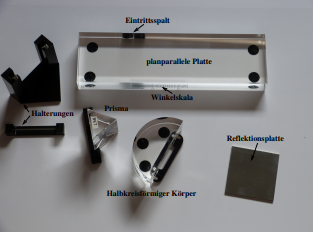
\includegraphics[width = 0.5\textwidth]{bilder/objekte.PNG}
            \caption{Die verschiedenen Objekte zur Untersucheung von Brechung und Reflexion.\cite{anleitung}}
            \label{fig:objekte}
        \end{figure}
        %\caption{Der Versuchsaufbau, die Gitter sind hier nicht zu sehen.}
